\section{实验}
\label{sec:experiments}

\subsection{实验设置}
\label{sec:setup}

主实验使用 LLaVA-1.5-7B~\cite{llava15}。高分辨率迁移预留 LLaVA-NeXT-7B 和 Qwen2.5-VL-7B，视频骨干与 LLaVA-OneVision-7B 的位置另表保留~\cite{llavanext,qwen25vl,onevision}。对比按依据分成三组，每组三种。交互注意力：FastV、SparseVLM、ViTCoP~\cite{fastv,sparsevlm,vitcop}。视觉代表：DART、DivPrune、SCoRe~\cite{dart,divprune,score}。联合选择：VisionZip、CoIn、PruneSID~\cite{visionzip,coin,prunesid}。小表每组取两种，视频表另加 FrameFusion~\cite{framefusion}。

图像任务是 GQA、POPE、MME、MMBench、ScienceQA-IMG、TextVQA-OCR，以及待补的 AI2D 和 VizWiz~\cite{gqa,pope,mme,mmbench,scienceqa,textvqa,ai2d,vizwiz}。POPE 报告 F1，MME 在主表和本轮六项里用感知分，分母 1510.70。其余分母为 GQA 61.90、POPE 85.80、MMBench 64.10、ScienceQA-IMG 69.51、TextVQA-OCR 58.20。相对分数是 $100\times$ 绝对分 $/$ 分母，Rel.6 与 Rel.8 是对应任务上这些比值的算术平均。样本数为 GQA 12578、POPE 9000、MME 2374、MMBench 4329、ScienceQA-IMG 2017、TextVQA-OCR 5000。双深度对照使用更早的四项协议，MME 为感知加认知，分母 1852，不能与感知分列混用。

评测在 NVIDIA V100 上用 lmms-eval 按单样本进行~\cite{lmmseval}。问题、选项和 OCR 提示按各任务协议进入语言模型。问题交换的方向只从问题句的内容词计算。层均容量 $\bar K=W/L$ 用来对齐一次剪枝和分层剪枝。主表三档是 $\bar K=128$、$64$、$32$，相对 576 个原始位置的 token-layer 预算分别减少 77.8\%、88.9\% 和 94.4\%。短横线表示该格还没有同协议记录。

\subsection{LLaVA-1.5-7B}
\label{sec:main}

\begin{table*}[t]
\centering
\scriptsize
\setlength{\tabcolsep}{3.2pt}
\caption{LLaVA-1.5-7B 八任务主结果。分组与三档预算沿用 SCoRe 的表式。MME 为感知分。Rel.6 只平均已有六项，Rel.8 在 AI2D 与 VizWiz 齐备后计算。短横线待填。}
\label{tab:main}
\begin{tabular}{@{}l r r r r r r r r r r@{}}
\hline
方法 & GQA & POPE & MME & MMB & SQA & Text & AI2D & Viz & Rel.6 & Rel.8 \\
\hline
\multicolumn{11}{@{}l}{完整模型，576 个视觉位置} \\
LLaVA-1.5-7B & 61.90 & 85.80 & 1510.70 & 64.10 & 69.51 & 58.20 & -- & -- & 100.00 & -- \\
\hline
\multicolumn{11}{@{}l}{$\bar K{=}128$，预算减少 77.8\%} \\
\multicolumn{11}{@{}l}{\enspace 交互注意力} \\
FastV~\cite{fastv} & -- & -- & -- & -- & -- & -- & -- & -- & -- & -- \\
SparseVLM~\cite{sparsevlm} & -- & -- & -- & -- & -- & -- & -- & -- & -- & -- \\
ViTCoP~\cite{vitcop} & -- & -- & -- & -- & -- & -- & -- & -- & -- & -- \\
\multicolumn{11}{@{}l}{\enspace 视觉代表} \\
DART~\cite{dart} & -- & -- & -- & -- & -- & -- & -- & -- & -- & -- \\
DivPrune~\cite{divprune} & -- & -- & -- & -- & -- & -- & -- & -- & -- & -- \\
SCoRe~\cite{score} & -- & -- & -- & -- & -- & -- & -- & -- & -- & -- \\
\multicolumn{11}{@{}l}{\enspace 联合选择} \\
VisionZip~\cite{visionzip} & -- & -- & -- & -- & -- & -- & -- & -- & -- & -- \\
CoIn~\cite{coin} & -- & -- & -- & -- & -- & -- & -- & -- & -- & -- \\
PruneSID~\cite{prunesid} & -- & -- & -- & -- & -- & -- & -- & -- & -- & -- \\
BELA & -- & -- & -- & -- & -- & -- & -- & -- & -- & -- \\
\hline
\multicolumn{11}{@{}l}{$\bar K{=}64$，预算减少 88.9\%} \\
\multicolumn{11}{@{}l}{\enspace 交互注意力} \\
FastV~\cite{fastv} & -- & -- & -- & -- & -- & -- & -- & -- & -- & -- \\
SparseVLM~\cite{sparsevlm} & -- & -- & -- & -- & -- & -- & -- & -- & -- & -- \\
ViTCoP~\cite{vitcop} & -- & -- & -- & -- & -- & -- & -- & -- & -- & -- \\
\multicolumn{11}{@{}l}{\enspace 视觉代表} \\
DART~\cite{dart} & -- & -- & -- & -- & -- & -- & -- & -- & -- & -- \\
DivPrune~\cite{divprune} & -- & -- & -- & -- & -- & -- & -- & -- & -- & -- \\
SCoRe~\cite{score} & -- & -- & -- & -- & -- & -- & -- & -- & -- & -- \\
\multicolumn{11}{@{}l}{\enspace 联合选择} \\
VisionZip~\cite{visionzip} & -- & -- & -- & -- & -- & -- & -- & -- & -- & -- \\
CoIn~\cite{coin} & -- & -- & -- & -- & -- & -- & -- & -- & -- & -- \\
PruneSID~\cite{prunesid} & -- & -- & -- & -- & -- & -- & -- & -- & -- & -- \\
BELA & -- & -- & -- & -- & -- & -- & -- & -- & -- & -- \\
\hline
\multicolumn{11}{@{}l}{$\bar K{=}32$，预算减少 94.4\%} \\
\multicolumn{11}{@{}l}{\enspace 交互注意力} \\
FastV~\cite{fastv} & -- & -- & -- & -- & -- & -- & -- & -- & -- & -- \\
SparseVLM~\cite{sparsevlm} & -- & -- & -- & -- & -- & -- & -- & -- & -- & -- \\
ViTCoP~\cite{vitcop} & -- & -- & -- & -- & -- & -- & -- & -- & -- & -- \\
\multicolumn{11}{@{}l}{\enspace 视觉代表} \\
DART~\cite{dart} & -- & -- & -- & -- & -- & -- & -- & -- & -- & -- \\
DivPrune~\cite{divprune} & -- & -- & -- & -- & -- & -- & -- & -- & -- & -- \\
SCoRe~\cite{score} & -- & -- & -- & -- & -- & -- & -- & -- & -- & -- \\
\multicolumn{11}{@{}l}{\enspace 联合选择} \\
VisionZip~\cite{visionzip} & -- & -- & -- & -- & -- & -- & -- & -- & -- & -- \\
CoIn~\cite{coin} & -- & -- & -- & -- & -- & -- & -- & -- & -- & -- \\
PruneSID~\cite{prunesid} & -- & -- & -- & -- & -- & -- & -- & -- & -- & -- \\
BELA & 57.08 & 86.19 & 1408.92 & 61.51 & 69.86 & 53.28 & -- & -- & 95.66 & -- \\
\hline
\end{tabular}
\end{table*}

表~\ref{tab:main} 里，94.4\% 这一档的 BELA 得到 GQA 57.08、POPE F1 86.19、MME 感知分 1408.92、MMBench 61.51、ScienceQA-IMG 69.86、TextVQA-OCR 53.28，Rel.6 为 95.66\%。ScienceQA 与 POPE 接近或超过各自参考，GQA 和 TextVQA 仍明显低于完整模型。外部方法和另外两档没有填入文献表里的数字：那些数字来自不同的保留定义、任务集合和 Dense 分母，不能与 $\bar K$ 直接并排。

\subsection{高分辨率迁移}
\label{sec:transfer}

LLaVA-NeXT 的切块和 Qwen2.5-VL 的动态分辨率会改变视觉序列长度，转移结果要用各模型自己的 Dense。表~\ref{tab:next} 和表~\ref{tab:qwen} 只保留六项经典任务。Signal 标的是方法的主要依据：Attn. 为交互注意力，Geom. 为特征几何，Sal.+Cov. 为显著性加覆盖，Hybrid 为联合准则，Stage 为入口构建后再分层执行。Qwen 的两档压缩率是 80.2\% 和 90.1\%。两张表的分数都还没有同协议记录。

\begin{table}[t]
\centering
\scriptsize
\setlength{\tabcolsep}{2.4pt}
\caption{LLaVA-NeXT-7B。六项经典任务，容量与分数待填。}
\label{tab:next}
\begin{tabular}{@{}llrrrrrr@{}}
\hline
方法 & Signal & GQA & POPE & MME & MMB & SQA & Text \\
\hline
Dense & Full & -- & -- & -- & -- & -- & -- \\
FastV~\cite{fastv} & Attn. & -- & -- & -- & -- & -- & -- \\
SparseVLM~\cite{sparsevlm} & Attn. & -- & -- & -- & -- & -- & -- \\
DivPrune~\cite{divprune} & Geom. & -- & -- & -- & -- & -- & -- \\
SCoRe~\cite{score} & Sal.+Cov. & -- & -- & -- & -- & -- & -- \\
CoIn~\cite{coin} & Hybrid & -- & -- & -- & -- & -- & -- \\
PruneSID~\cite{prunesid} & Hybrid & -- & -- & -- & -- & -- & -- \\
BELA & Stage & -- & -- & -- & -- & -- & -- \\
\hline
\end{tabular}
\end{table}

\begin{table}[t]
\centering
\scriptsize
\setlength{\tabcolsep}{2.4pt}
\caption{Qwen2.5-VL-7B。上块减少 80.2\% 的视觉预算，下块减少 90.1\%。分数待填。}
\label{tab:qwen}
\begin{tabular}{@{}llrrrrrr@{}}
\hline
方法 & Signal & GQA & POPE & MME & MMB & SQA & Text \\
\hline
\multicolumn{8}{@{}l}{压缩 80.2\%} \\
Dense & Full & -- & -- & -- & -- & -- & -- \\
FastV~\cite{fastv} & Attn. & -- & -- & -- & -- & -- & -- \\
SparseVLM~\cite{sparsevlm} & Attn. & -- & -- & -- & -- & -- & -- \\
DivPrune~\cite{divprune} & Geom. & -- & -- & -- & -- & -- & -- \\
SCoRe~\cite{score} & Sal.+Cov. & -- & -- & -- & -- & -- & -- \\
CoIn~\cite{coin} & Hybrid & -- & -- & -- & -- & -- & -- \\
PruneSID~\cite{prunesid} & Hybrid & -- & -- & -- & -- & -- & -- \\
BELA & Stage & -- & -- & -- & -- & -- & -- \\
\hline
\multicolumn{8}{@{}l}{压缩 90.1\%} \\
FastV~\cite{fastv} & Attn. & -- & -- & -- & -- & -- & -- \\
SparseVLM~\cite{sparsevlm} & Attn. & -- & -- & -- & -- & -- & -- \\
DivPrune~\cite{divprune} & Geom. & -- & -- & -- & -- & -- & -- \\
SCoRe~\cite{score} & Sal.+Cov. & -- & -- & -- & -- & -- & -- \\
CoIn~\cite{coin} & Hybrid & -- & -- & -- & -- & -- & -- \\
PruneSID~\cite{prunesid} & Hybrid & -- & -- & -- & -- & -- & -- \\
BELA & Stage & -- & -- & -- & -- & -- & -- \\
\hline
\end{tabular}
\end{table}

\subsection{视频理解}
\label{sec:video}

视频表预留四个基准：LongVideoBench、Video-MME、LVE，以及名称尚未确认的第四项~\cite{longvideobench,videomme}。LVE 的全称待核对后再补引用。比较对象包括表~\ref{tab:video} 中的图像方法，以及面向帧间重复的 FrameFusion。帧标记、时间标记和图像 patch 分开计数。这一节没有填入分数。

\begin{table}[t]
\centering
\scriptsize
\setlength{\tabcolsep}{3pt}
\caption{视频理解。同骨干、同帧采样下比较。四列都待填。}
\label{tab:video}
\begin{tabular}{@{}lrrrr@{}}
\hline
方法 & LongVB & V-MME & LVE & 第四项 \\
\hline
Dense & -- & -- & -- & -- \\
FastV~\cite{fastv} & -- & -- & -- & -- \\
SparseVLM~\cite{sparsevlm} & -- & -- & -- & -- \\
DivPrune~\cite{divprune} & -- & -- & -- & -- \\
SCoRe~\cite{score} & -- & -- & -- & -- \\
CoIn~\cite{coin} & -- & -- & -- & -- \\
PruneSID~\cite{prunesid} & -- & -- & -- & -- \\
FrameFusion~\cite{framefusion} & -- & -- & -- & -- \\
BELA & -- & -- & -- & -- \\
\hline
\end{tabular}
\end{table}

\subsection{效率}
\label{sec:efficiency}

效率还没有测量。计划在同一张 V100 上，对 Dense、一种交互基线、一种覆盖基线、关闭问题交换的 BELA 和完整 BELA，使用相同图像、批量 1 和精度。准确率评测按任务自然停止。计时另用固定生成长度，避免答案长短混进延迟。端到端首 token 时间从已经载入的图像和文本算起，包含视觉塔、投影、选择和预填充，直到第一个生成 token 可用。同时记录这段生成的总时间和峰值显存。模块计时分开看视觉塔、全网格投影、双深度与配额、问题交换，以及剪点上的问题--键乘积。预热不计入稳态。每个配置重复数轮，报告中位数、均值和尾部。相同的 $W$ 只说明视觉 token-layer 数量相同，加速比以这组计时为准。表~\ref{tab:eff} 留待填入。

\begin{table}[t]
\centering
\scriptsize
\setlength{\tabcolsep}{3pt}
\caption{效率位置。同设备、同输入、固定生成长度。数字待测。}
\label{tab:eff}
\begin{tabular}{@{}lrrrr@{}}
\hline
方法 & TTFT & 生成时间 & 峰值显存 & 加速比 \\
\hline
Dense & -- & -- & -- & 1.00 \\
SCoRe~\cite{score} & -- & -- & -- & -- \\
CoIn~\cite{coin} & -- & -- & -- & -- \\
BELA，交换关 & -- & -- & -- & -- \\
BELA & -- & -- & -- & -- \\
\hline
\end{tabular}
\end{table}

\subsection{消融}
\label{sec:ablation}

\begin{figure*}[t]
\centering
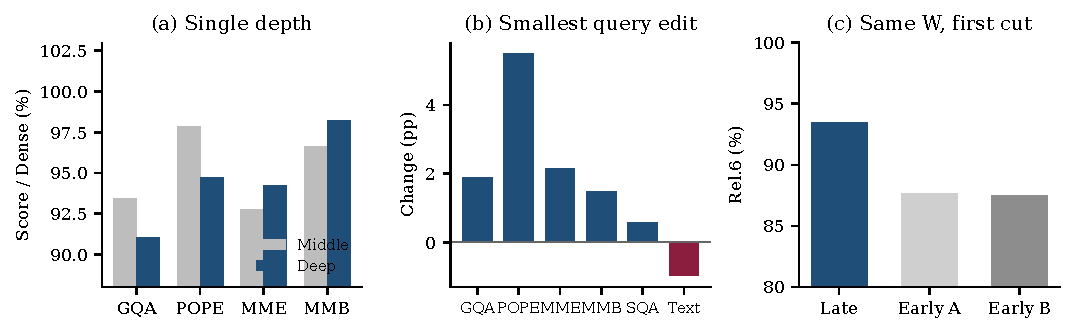
\includegraphics[width=\textwidth]{figures/observations.pdf}
\caption{三组已经分开的观察。（a）关闭问题交换时，中层与深层的四项相对分各有高低，MME 用总分。（b）格子配额基底上，最小一档交换的相对分变化；TextVQA 为负。（c）同一个 $W$ 下，第一次收缩较晚的 Rel.6 更高，MME 用感知分。三幅图的分母不完全相同。}
\label{fig:obs}
\end{figure*}

双深度对照来自更早的 $W{=}2048$ 协议，问题交换关闭，MME 用总分，所以不能和表~\ref{tab:main} 的 95.66\% 写成同一预算。中层在 GQA 和 POPE 上最高，深层在 MMBench 上最高，双深度加旧覆盖在 MME 和四项相对均值上最高，见表~\ref{tab:depth}。GQA 上双深度低于只使用中层。MMBench 全量里，中层对、深层错、双深度对的有 35 题；深层对、中层错、双深度也错的有 38 题。双深度提供的是两套排序，不是每个任务上的更优深度。

\begin{table}[t]
\centering
\scriptsize
\setlength{\tabcolsep}{3pt}
\caption{双深度。问题交换关闭，MME-T 为总分，Rel.4 只用这四项。}
\label{tab:depth}
\begin{tabular}{@{}lrrrrr@{}}
\hline
引导 & GQA & POPE & MME-T & MMB & Rel.4 \\
\hline
中层 & 57.84 & 83.97 & 1718.0 & 61.94 & 95.18 \\
深层 & 56.34 & 81.28 & 1745.7 & 62.97 & 94.56 \\
双深度 & 57.33 & 82.77 & 1744.5 & 62.54 & 95.22 \\
双深度+旧覆盖 & 57.18 & 82.99 & 1765.2 & 62.20 & 95.36 \\
\hline
\end{tabular}
\end{table}

覆盖变体固定双深度并关闭问题交换，使用本轮六项和感知分。只修正空格与负余弦时，Rel.6 从 93.47\% 变为 93.50\%。去掉空格候选的显著性后，POPE 降到 76.33，Rel.6 降到 90.96\%。格子配额在这组里最高，为 93.89\%，MME 感知分和 TextVQA 上升，POPE 与 MMBench 下降。逐步更新原型是 93.77\%，把残差放宽到锚点之外是 93.27\%。完整六行见附录。

在格子配额上打开问题交换，最小一档把 Rel.6 从 93.89\% 提高到 95.66\%。旧覆盖加同一档交换是 95.29\%，低于这一组合。GQA 从 55.92 到 57.08：由错到对 498 题，由对到错 353 题，净增 145 题。POPE F1 从 81.48 到 86.19，TextVQA 从 53.85 到 53.28。再增大交换上限，POPE 继续上升，MME、MMBench、ScienceQA 和 TextVQA 一起下降，Rel.6 依次为 94.78\%、93.68\% 和 93.02\%。最小一档是这四档里的六项最高值，上限本身是任务取舍，不是越大越好。

同一个 $W{=}1024$ 下，第一次收缩较晚的 Rel.6 为 93.47\%，两次较早收缩为 87.67\% 和 87.45\%。晚收缩那一档的入口个数更小，分数反而更高。这三档同时改变了入口容量和各档维持的层数，不能单独画成“入口越小越差”。历史中间档在另一套四项协议上，中间过少为 92.76\%，中间适中为 95.36\%，中间很多但很快掉到最终档为 94.56\%；维持层数和中间个数也绑在一起。前两档相同、只改最后两档时，Rel.6 为 96.78\% 和 96.89\%，相差 0.11 个百分点。深层已经走过之后，所比较的末段分配对均值影响很小。具体保留序列和层数写在附录，不写入方法定义。

\begin{figure}[t]
\centering
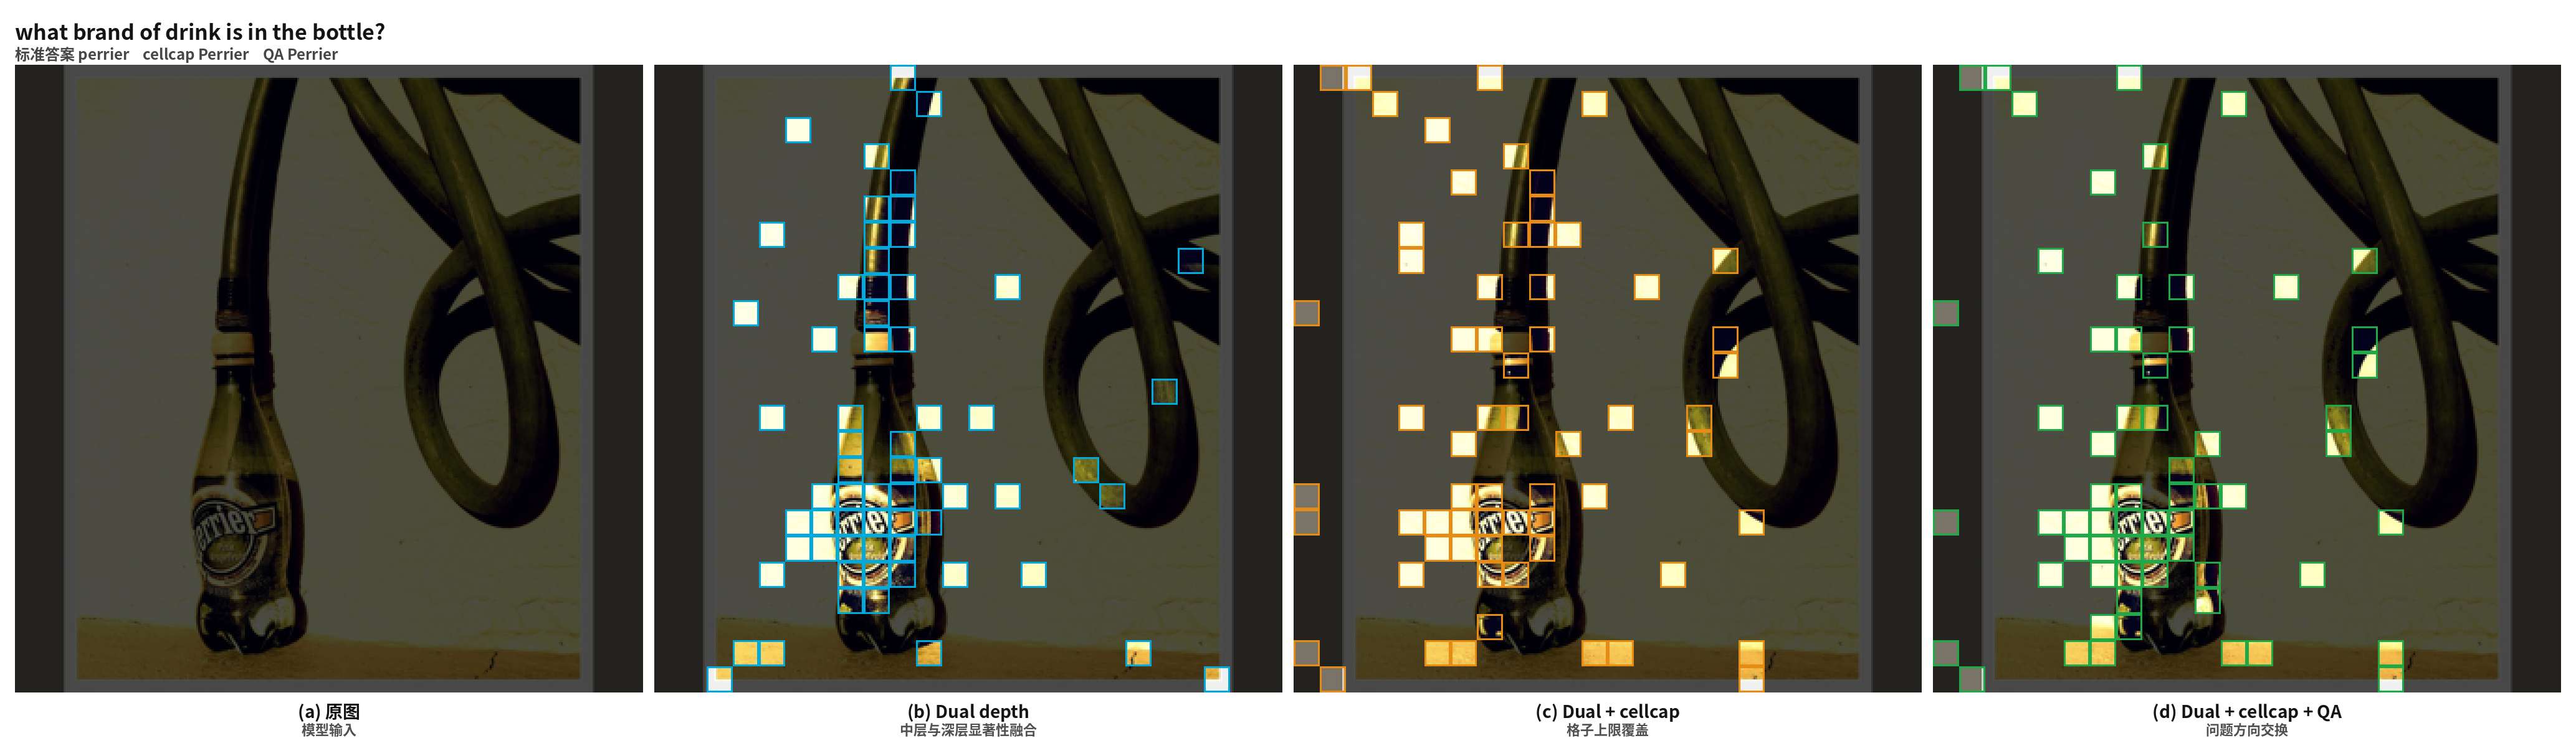
\includegraphics[width=\linewidth]{figures/textvqa_bottle.png}
\caption{TextVQA：瓶身商标。未选区域压暗，选中 patch 保持原亮度。（b）（c）（d）来自同一次前向。配额与日志逐格重合。格子配额和问题交换都回答 Perrier。}
\label{fig:bottle}
\end{figure}

图~\ref{fig:bottle} 用半栏放进同一次前向的四联保留图。问题是瓶身饮料品牌，标准答案为 Perrier。问题交换把一部分亮块从水管移到商标附近。钟楼与无手套两例用同样的半栏尺寸放在附录：钟楼金标为 B，两种入口都答 B；无手套一例两边都答 No，只说明亮块从救生圈文字移到下方人物，图中没有手套。旧的按数据集行号叠上去的图没有使用，因为当时的轨迹按问题长度排序，格子和图像不是同一次前向。
